\chapter{Approach}

\section{System Overview}

The overall system design is shown at Figure \ref{fig:overview}.

\begin{figure}[!htb]
    \centering
    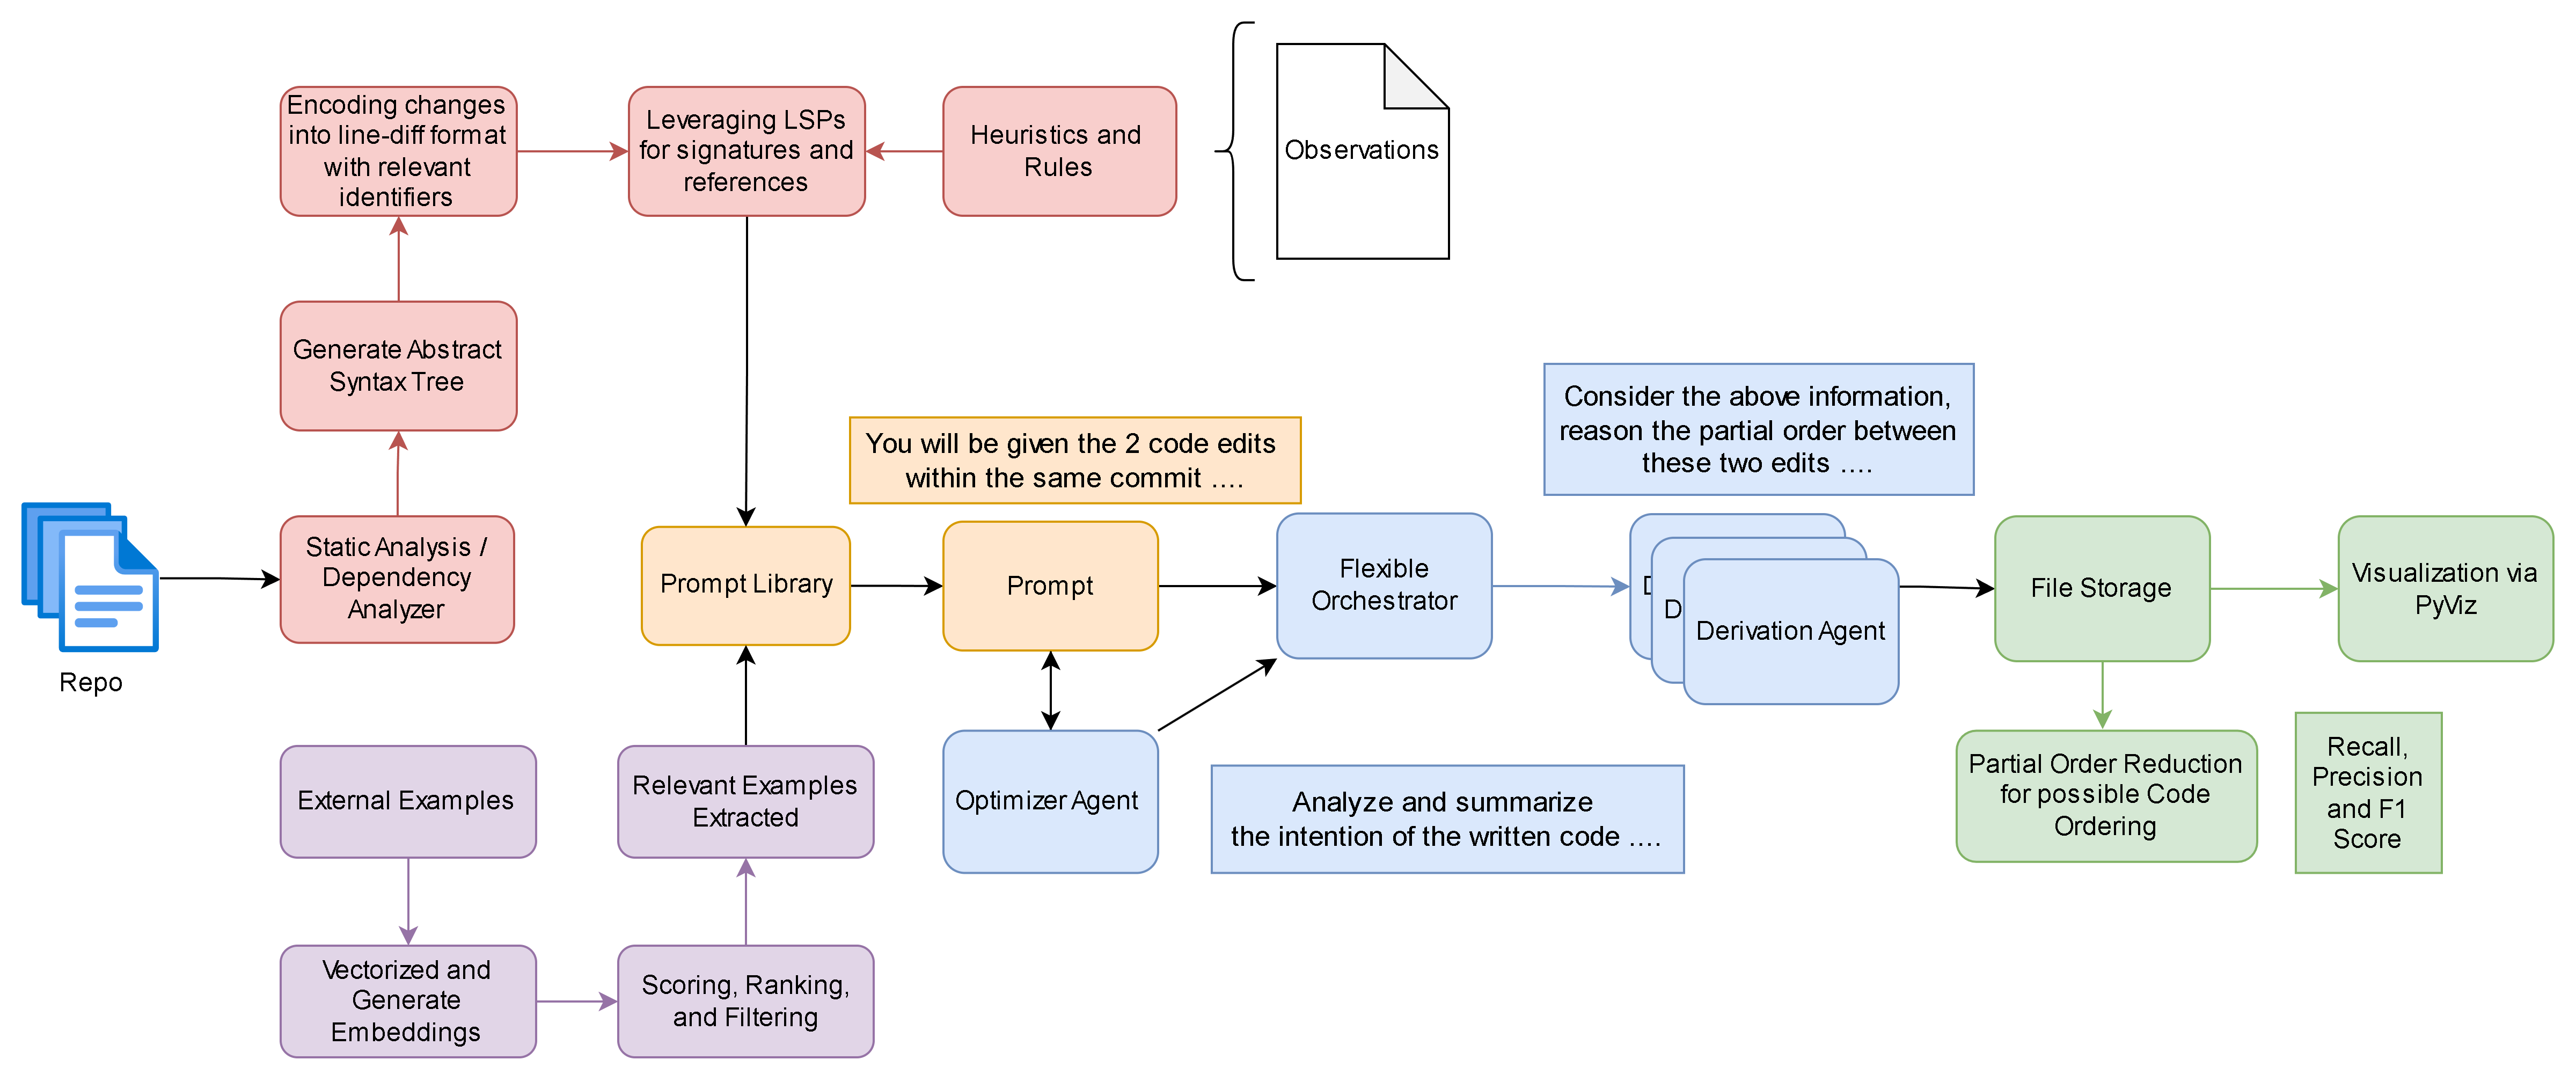
\includegraphics[width=1\linewidth]{fig/overview.png}
    \caption{System Overview}
    \label{fig:overview}
\end{figure}

\section{Encoding Code Changes}

We use a line-diff-based format to encode code changes. Let \( u \) represent a code block composed of lines \( l_1, l_2, \dots, l_m \), with an edit region spanning lines \( l_a \) through \( l_{a+n} \), where \( 1 \leq a \leq a + n \leq m \). For each line \( l_i \) within this range, we associate a status variable \( s_i \) to indicate the type of change applied. The status variable \( s_i \) is defined as follows:

\[
s_i = 
\begin{cases} 
    + & \text{if line \( l_i \) is an addition,} \\
    - & \text{if line \( l_i \) is a deletion,} \\
    = & \text{if line \( l_i \) is unchanged (optional).}
\end{cases}
\]

In addition to line-specific information, each edit region \( R \subseteq u \) is also annotated with contextual metadata, including the file path, denoted as \( p(u) \), and the logic path, denoted as \( \ell(u) \). The logic path \( \ell(u) \) represents the hierarchical structure of the code, encompassing the local block, any enclosing blocks, and the parent block. An example is shown below.

\begin{figure}[h]
\scriptsize
\begin{minted}[breaklines, frame=lines]{python}
--- src/transformers/commands/run.py
+++ src/transformers/commands/run.py

@@61,3 61,1 @@ class RunCommand(BaseTransformersCLICommand): >>>> def register_subcommand(parser: ArgumentParser)

@staticmethod
def register_subcommand(parser: ArgumentParser):
    run_parser = parser.add_parser("run", help="Run a pipeline through the CLI")
-   run_parser.add_argument(
-       "--task", choices=list(SUPPORTED_TASKS.keys()) + list(TTASK_ALIASES.keys()), help="Task to run"
-   )
+   run_parser.add_argument("--task", choices=get_supported_tasks(), help="Task to run")
    run_parser.add_argument("--input", type=str, help="Path to the file to use for inference")
    run_parser.add_argument("--output", type=str, help="Path to the file for writing results post-inference.")
    run_parser.add_argument("--model", type=str, help="Name or path to the model to instantiate.")
\end{minted}
\caption{Encoding code change in src/transformers/commands/run.py}
\label{code:encoded_code_change}
\end{figure}

\begin{figure}
    \centering
    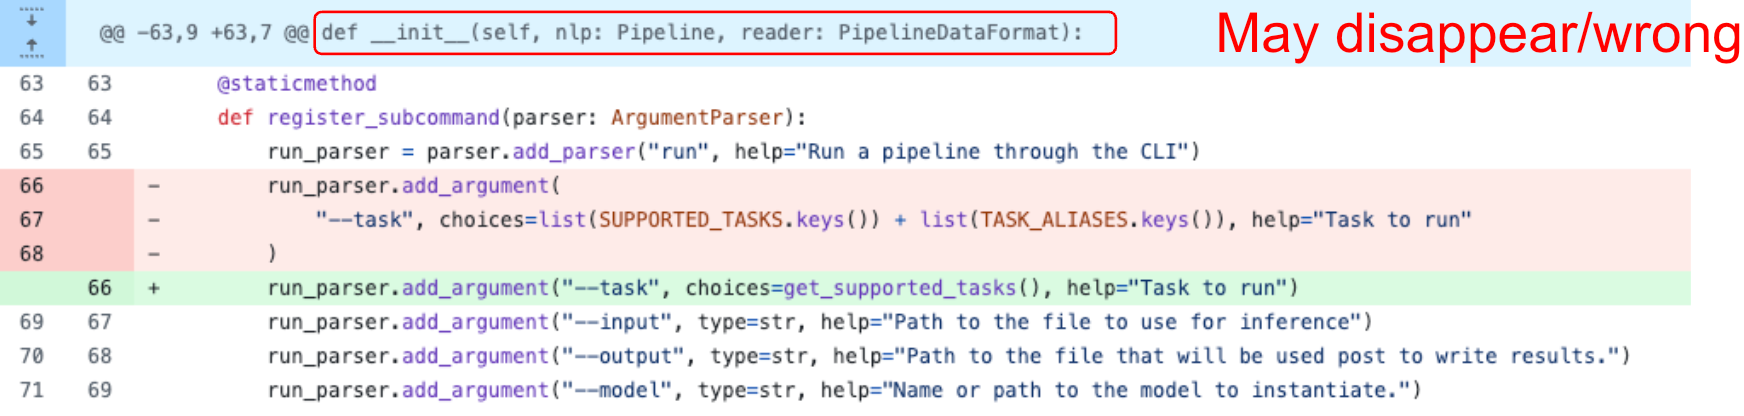
\includegraphics[width=1\linewidth]{fig/encode.png}
    \caption{Original edit span in src/transformers/commands/run.py}
    \label{fig:original_code_change}
\end{figure}

% \section{Analyzing Relevant Signatures}

% With our method for encoding code changes in place, we also need an efficient approach for inputting \( U \), the remaining codebase, into the model. Inputting the entire codebase directly would generate an excessive number of tokens, overwhelming the model’s context window. Instead, we use lightweight static analysis to extract only the most relevant information for context enhancement.

% For each target code region \( u \), we analyze its pre-edit code and compile a list of its usages. For function usages, we extract the function signature; for variables or class members, we retrieve the initial assignment statement. These extracted signatures and usage statements are then concatenated into a single document, serving as supplementary context for the model to interpret dependencies and relationships more accurately.


\section{Multi-Agent Validation}

We define a multi-staged multi-agent system \( \mathcal{A} = \{ A_1, A_2, \dots, A_k \} \), where each agent \( A_i \) is responsible for validating and deducing dependencies for a subset of edit representations \( E_i \subseteq \mathbf{H} \), with \( \mathbf{H} \) being the complete set of edits. Each agent operates independently to analyze the dependencies within its assigned subset \( E_i \) and communicates findings with other agents in the system to achieve consensus on the ordering relationships.

\subsubsection{Stage 1: Optimizer Agent: Information Integration and Summarization}

% In Stage 1, the optimizer agent extracts relevant information in a long-context source and synthesizes relevant information accumulated to generate the response.


% \subsubsection{Stage 2: Worker Agent: Segment Comprehension}

% For each edit representation \( h_j \in E_i \), agent \( A_i \) examines contextual and structural information—encoded as features \( \mathbf{f}(h_j) \)—to determine potential dependencies with other edits \( h_k \in \mathbf{H} \).

% Each agent \( A_i \) thus outputs a set of dependency relationships \( R_i = \{ R(h_j, h_k) \mid h_j, h_k \in E_i \} \), which collectively represent the inferred ordering within its subset. Agents then perform inter-agent validation by communicating these relationships, enabling consensus-building across all subsets \( E_1, E_2, \dots, E_k \). The combined results from all agents form the global dependency graph \( G = (\mathbf{H}, E) \), where \( E \) contains directed edges representing dependencies across all edits.

% By employing a multi-agent approach, this system can efficiently validate complex dependency structures and deduce partial ordering across large sets of edits, enhancing the accuracy and scalability of the ordering inference process.

% \begin{algorithm}
% \caption{Chain of Agents (CoA)}
% \label{alg:coa}
% \begin{algorithmic}[1]
% \Require Source input $x$, query $q$, agent window size $k$, large language model $\text{LLM}(\ast)$.
% \Ensure Answer to the query.
% \State Split $x$ into $l$ chunks $\{c_1, c_2, \dots, c_l\}$ where $c_i$ is shorter than $k$
% \State Initialize $CU_0 \gets$ empty string.
% \For{$i \in \{1,2,\dots,l\}$}
%     \State $CU_i \gets \text{LLM}_{W_i}(I_W, CU_{i-1}, c_i, q)$
% \EndFor
% \State \textbf{return} $\text{LLM}_M(I_M, CU_l, q)$
% \end{algorithmic}
% \end{algorithm}

The optimizer agent operates on the initial set of code edits \( \mathbf{H} \) and aims to condense and structure the available information. Given an input sequence of code modifications, the agent performs the following tasks:

\begin{enumerate}
    \item \textbf{Intent Extraction}: The agent identifies the core intention behind each modification by leveraging large language models (LLMs) to summarize the logical changes, distinguishing between functional enhancements, bug fixes, and refactorings.
    \item \textbf{Pruned Information Output}: Redundant or irrelevant modifications (such as minor formatting changes) are filtered out to ensure a focused summary that retains only information critical to dependency resolution.
\end{enumerate}

Once the optimizer agent has synthesized the high-level description and intention of the code edits, the resulting structured representation is then passed forward to the next stage.

\subsubsection{Stage 2: Segmentation and Distributed Dependency Resolution}

Following the summarization phase, the second stage focuses on decomposing the summarized code changes into smaller, independent segments. This segmentation process is crucial for enabling parallelized dependency analysis across multiple worker agents.

\paragraph{Contextual Segmentation}
The system partitions the summarized code modifications into independent code regions. Given an initial summary \( S \) generated by the optimizer agent, the segmentation module groups the edits into disjoint subsets:
\[
\mathcal{S} = \{ S_1, S_2, \dots, S_n \}, \quad S_i \subseteq S
\]
where each subset \( S_i \) represents a logically independent code fragment. The segmentation criteria are based on:
\begin{itemize}
    \item Scope of the modification (e.g., function, class, or module level)
    \item Interdependencies derived from the call graph and symbol resolution
    \item Heuristic-based clustering using textual and semantic similarity measures
\end{itemize}

\paragraph{Worker Agents: Dependency Inference}
Each segmented context \( S_i \) is independently assigned to a worker agent \( A_i \), which evaluates dependencies between code changes within its assigned context. The dependency inference operates as follows:

\begin{enumerate}
    \item \textbf{Pairwise Comparison}: For each code edit pair \( (e_i, e_j) \in S_i \), the agent determines the relationship \( \mathcal{R}(e_i, e_j) \) by assessing lexical, syntactic, and semantic dependencies.
    \item \textbf{Partial Order Estimation}: The agent constructs a local dependency graph \( G_i \) capturing directed relationships between dependent edits:
    \[
    G_i = (V_i, E_i), \quad \text{where } V_i = S_i \text{ and } E_i = \{ (e_x, e_y) \mid e_x \text{ must precede } e_y \}
    \]
    \item \textbf{Inter-Agent Communication}: Worker agents exchange boundary dependencies where segmented contexts overlap. If an edit \( e_x \) in one subset \( S_a \) influences an edit \( e_y \) in another subset \( S_b \), a cross-agent dependency edge is introduced: \( (e_x, e_y) \in E \).
\end{enumerate}

\paragraph{Dependency Graph Construction}
After all worker agents complete their independent dependency resolution, the local dependency graphs \( G_1, G_2, \dots, G_n \) are aggregated into a global dependency graph:
\[
G = \bigcup_{i=1}^{n} G_i
\]
This final graph encodes the inferred ordering constraints across all code edits, enabling structured application of changes in a manner that preserves logical consistency and correctness.

\subsubsection{Consensus Mechanism and Final Ordering}

To ensure robustness in dependency determination, we introduce a consensus mechanism where conflicting dependencies reported by different agents are reconciled. This is achieved through:

\begin{itemize}
    \item \textbf{Voting-Based Resolution}: If multiple agents provide conflicting orderings for a given edit pair, a majority vote determines the final ordering.
    \item \textbf{Confidence-Weighted Merging}: Dependency edges with higher confidence scores—determined by the strength of inferred relationships—are prioritized.
    \item \textbf{Cycle Detection and Resolution}: The merged dependency graph is checked for cyclic dependencies, which are resolved through a priority-based tie-breaking strategy.
\end{itemize}

The final output of the multi-agent system is an optimized, globally consistent dependency graph that provides a structured execution plan for code modifications.

